\paragraph{}
GraphQL ist eine Abfragesprache und Server-Laufzeitumgebung für APIs. Diese dient dazu, die Daten zu liefern, die anfordert werden.
\\\\
Im Hinblick auf die Art und Weise, wie Abfragen an den Server mithilfe von GraphQL behandelt werden können, sind folgende Aspekte zu beachten.
\subsubsection*{Eigenschaften}
  \begin{itemize}
    \item
          GraphQL-Aufrufe werden in einem einzigen Round Trip gehandhabt.% Wir bekommen genau die Daten, die angefragt haben (kein Over-Fetching).

    \item
          Stark definierte Datentypen, welche das Risiko einer Fehlkommunikation zwischen Client und Server verringern.

    \item
          Eine Anwendungs-API kann sich mit GraphQL weiterentwickeln, ohne dass bestehende Abfragen beeinträchtigt werden.
    \item
          GraphQL schreibt keine spezifische Anwendungsarchitektur vor. Es kann auf einer vorhandenen REST-API installiert und mit aktuellen API-Management-Tools verwendet werden.
    \item
          Als Alternative zu REST ermöglicht GraphQL Entwicklern die Erstellung von Abfragen zur Extraktion von Daten aus mehreren Quellen mit einer einzigen API-Abfrage.

  \end{itemize}
  
  \subsection{Anforderungen und Technologiewahl}
Die Webseite besteht aus statischen und dynamischen Inhalten.
Statische Inhalte wie beispielsweise die Menuführung, liegen offen in einem HTML-Dokument und werden bei Abfrage der Webseite gesendet. 
Dynamische Inhalte, unter anderem Profile, Chats und Nachrichten, werden mit Daten aus der Datenbank gefüllt.
Um diese Daten bereitstellen zu können, ist eine Schnittstelle zwischen Datenbank und Frontend notwendig. 

Es wurde sich für GraphQL statt einer standardmäßigen REST-Schnittstelle entschieden.
GraphQL bietet verschiedene Verbesserungen, wie zum Beispiel Leistungsoptimierungen durch Overfetching und Underfetching, Stabilität durch ein Typenschema und Selbstdokumentation.

\subsection{Overfetching und Underfetching}
\paragraph{}
Da bei REST-Schnittstellen nicht wählbar ist, welche Daten in einer Abfrage zurückgegeben werden sollen, gibt es Abfragen, bei denen irrelevante Daten zurückgegeben werden.
Dies wird als Overfetching bezeichnet.
In einigen Fällen werden außerdem Daten benötigt, die mehrere Anfragen an verschiedene Endpunkte voraussetzen.
Dies wird als Underfetching bezeichnet.
Sowohl Overfetching als auch Underfetching sorgen für suboptimale Abfragen und es kommt zu Leistungseinbußen, entweder durch unnötig viel benötigte Bandbreite oder unnötige viele Abfragen.
Dieses Problem ist mit REST-Schnittstellen schwer zu umgehen, da es Praxisfern ist, für jede mögliche kombination von benötigten Daten einen perfekten Endpunkt zu erstellen.

\paragraph{}
GraphQL löst das Problem, indem bei jeder Anfrage genau definiert wird, welche Daten von welchen Endpunkten erfragt werden.
Neben genannter Leistungsoptimierung wird auch die Arbeit der Frontend-Endwickler erleichtert, da diese bei einer Abfrage genau die benötigten Daten definieren können - irrelevante Daten müssen gar nicht erst abgefragt werden, die Anfrage wird \enquote{verschlankt}.\\
REST fokussiert sich auf die verschiedenen Endpunkte, während GraphQL den Fokus auf die einzelnen Aufgaben legt.
In GraphQL entscheidet die Applikation über die Daten die es erhält, nicht der Server.
Mehrere Abfragen können in eine einzige Schnittstellenabfrage gebündelt werden, der Client erhält somit zusammenhängende Daten und die Datenbank wird durch präzise Abfragen geschont.

\subsection{Stabilität}
Durch GraphQls Typenschemata wird definiert, welche Abfragen und Mutationen möglich sind.
GraphQL akzeptiert Anfragen nur, wenn die richtigen Datentypen verwendet werden und weist fehlerhafte Anfragen zurück.
Sollte die Datenbank den falschen Datentyp zurückgeben, wird auch ein Fehler geworfen.
Der Klient kann somit bei einer Abfrage damit rechnen, Daten in den angegebenen Datentypen zu erhalten, Ausnahmen für andere Datentypen müssen nicht definiert werden.
Ebenso wird eine Abfrage mit nicht erlaubten Datentypen direkt mit einer Fehlermeldung beantwortet, die genau auf den falschen Datentyp hinweist.
Dadurch werden Inkonsistenzen der Datenbank und der Zwang für weitere Datentypenkontrollen durch Design bereits stark mitigiert.

\subsection{Dokumentation}
GraphQL selbstdokumentiert jeden Endpunkt durch die vorliegenden Datentypen.
Bei Änderungen an der Schnittstelle wird die Dokumentation automatisch aktualisiert. Auch kann manuell eine Beschreibung des Endpunkts hinzugefügt werden. Dies erleichtert es dem Frontend, die richtigen Endpunkte und Datentypen für Abfragen und Mutationen zu verwenden. Durch die angegebenen Datentypen ist das Frontend in der Lage, direkt zu erkennen, welche Datentypen in der entsprechenden Abfrage oder Mutation zu verwenden sind und kann damit Zeit sparen.
Gleichzeitig fällt Zeit weg, die für das manuelle Dokumentieren der Schnittstelle angefallen wäre.

\subsection{GraphiQL}
Mit GraphiQL liefert GraphQL einen Webeditor, der das Schreiben von Abfragen und Mutationen vereinfacht.
Der Editor liefert einige Funktionen, die den Umgang einfacher machen, wie zum Beispiel automatisches Komplettieren von Variablennamen oder das Formatieren in eine lesbarere Struktur.
Der Editor hat außerdem Zugriff auf die Typenschemata und Dokumentation und kann damit Abfragen auf syntaktische Fehler untersuchen, noch bevor diese abgeschickt werden.
Der Editor steht unter der Route \textit{/graphql} für jeden Nutzer zur freien Verfügung und erleichtert somit die Arbeit für alle Programmierer, die unsere Schnittstelle verwenden.
Im Projekt konnte durch die Nutzung des Editors beim Erstellen von Datentypdefinitionen, Abfragen und Mutationen Programmierzeit gespart werden.

\begin{figure}
	\centering
    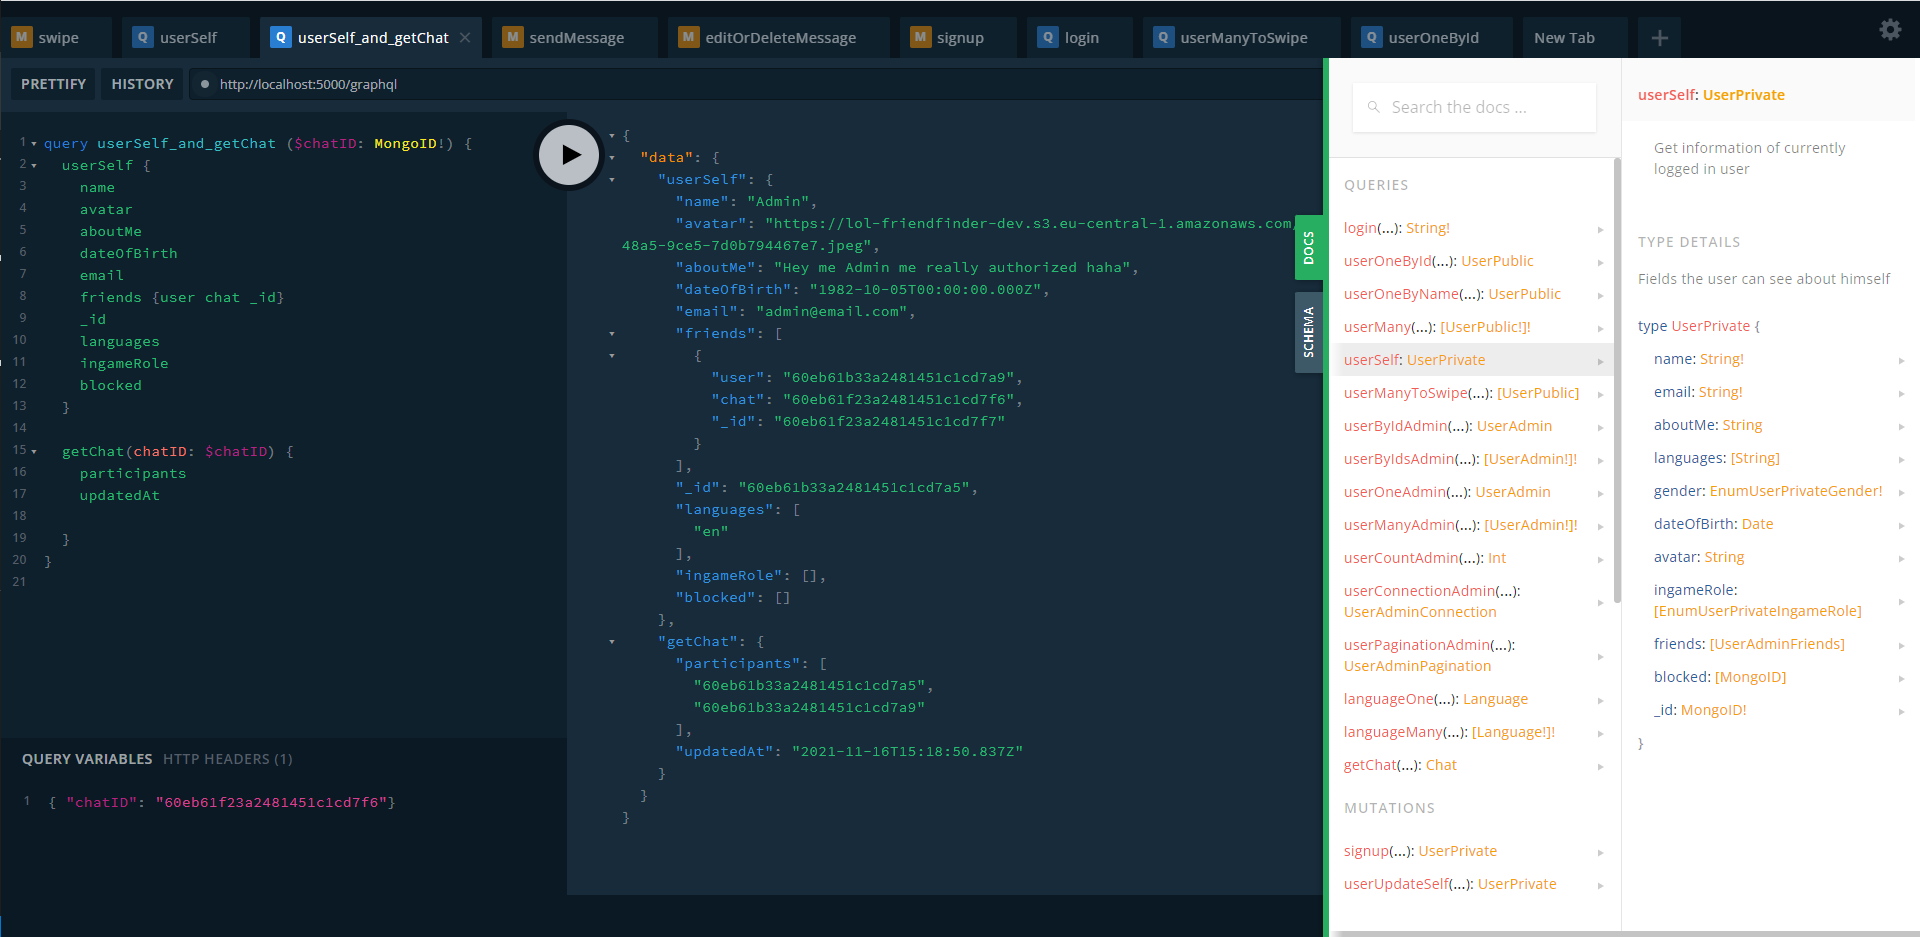
\includegraphics[width=\textwidth]{sources/graphiql.png}\cite{}
	\caption{GraphiQL Benutzeroberfläche. Links: Zwei Endpunkte werden durch eine Abfrage gebündelt abgefragt. Mitte: Antwort der Endpunkte. Rechts: Dokumentation und Typendefinition des Endpunkts \textit{userSelf}.}
	\label{fig:gql:1}
\end{figure}

\subsection{Resolver}
Durch die Pakete \textit{graphql-compose} und \textit{graphql-compose-mongoose} werden aus den bestehenden Datenbankmodellen Typenschemata entsprechend der Datentypen erstellt, die in GraphQL weiterverwendet werden können. 
Resolver ("to resolve", etw. auflösen/abwickeln/klären) beantworten Abfragen und Mutationen.
Sie bilden das Bindeglied zwischen Schnittstellenabfrage und Datenbankantwort. \\

\begin{figure}
	\centering
    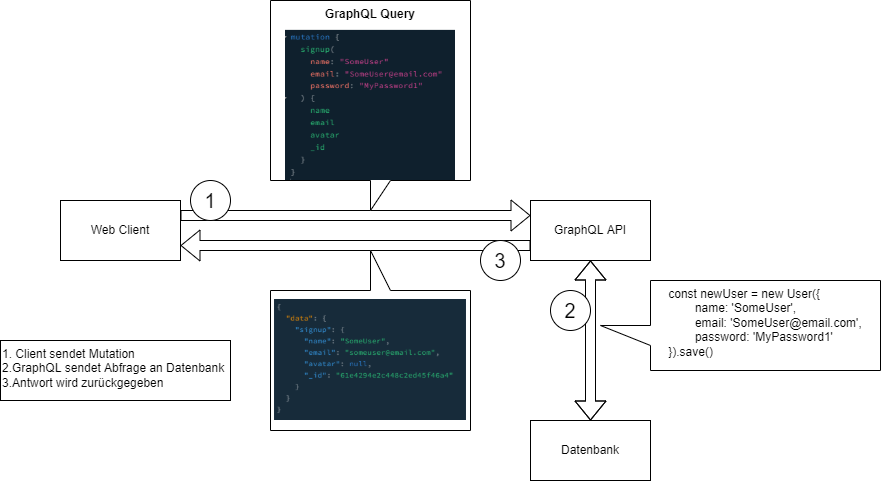
\includegraphics[width=\textwidth]{sources/GraphQL_Resolver_Schaubild.drawio}\cite{}
	\caption{Client sendet Abfrage an Resolver, dieser \enquote{übersetzt} Abfrage in Datenbanksprache und antwortet mit den Daten der DB}
	\label{fig:gql:resolver_schaubild}
\end{figure}

Simplere Resolver, welche zum Beispiel einen einzelnen Datenbankeintrag durch die ID identifizieren (\textit{findOne}) oder anhand der bestehenden Datenstruktur einen Datenbankeintrag erstellen (\textit{createOne}), werden durch die verwendeten Pakete bereit gestellt und lassen sich in das Projekt integrieren.
Für komplexere Resolver lassen sich bestehende Resolver anpassen oder gänzlich neue erstellen.
Die verwendeten Resolver und Typenschemata werden dem \textit{schemaComposer} bereit gestellt, welcher aus den bestehenden Daten die Dokumentation generiert.


\subsection{Verwendete Abfragen und Mutationen}
\paragraph{}
Nachfolgend werden einige der verwendeten Abfragen und Mutationen exemplarisch vorgestellt.

\paragraph{}
Für den Registrierungsvorgang wird die Mutation \textit{signup} verwendet.
Durch die Angabe von Email, gewünschtem Namen und Passwort wird ein Nutzerkonto erstellt.
In Zukunft kann durch Angabe von Namen und Passwort mit der \textit{login} Abfrage ein Authentifizierungstoken erstellt werden. Das Token wird bei Abfragen, die eine Authentifizierung oder Authorisierung verlangen, verwendet.

\begin{figure}
	\centering
    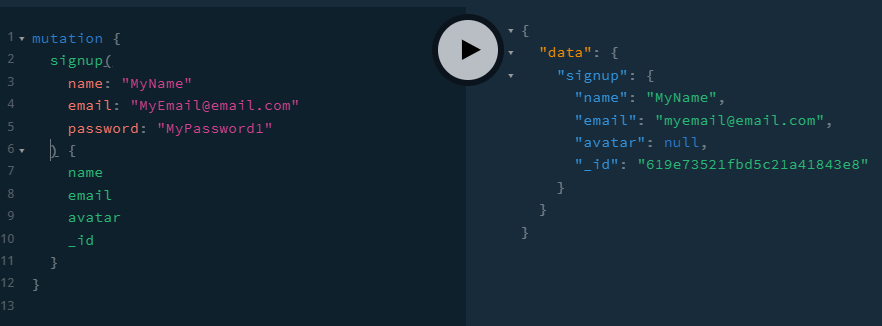
\includegraphics[width=\textwidth]{sources/graphiql_signup.png}
	\caption{Registrierung des neuen Nutzers \textit{MyName}. Eigene Darstellung.}
	\label{fig:gql:2}
\end{figure}

\begin{figure}
	\centering
    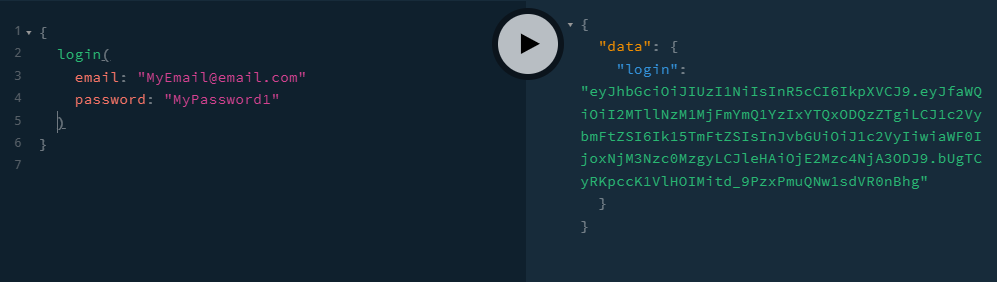
\includegraphics[width=\textwidth]{sources/graphiql_login.png}
	\caption{Anmeldung des Nutzers. Die Antwort enthält das JSON Web Token, welches für bestimmte Abfragen zur Authentifizierung und Autorisierung dient. Eigene Darstellung.}
	\label{fig:gql:3}
\end{figure}

\paragraph{}
Alle weiteren vorgestellten Endpunkte benötigen zur eindeutigen Indentifizierung ein valides Authentifizierungstoken.

\paragraph{}
Um das eigene Profil anzuzeigen, wird die \textit{userSelf} Abfrage verwendet.
Diese zeigt Daten entsprechend des Datenbankschemas an.
Einige dieser Daten sind veränderbar, so zum Beispiel der Freitext.
Zum Verändern der Daten ist die Mutation \textit{userUpdateSelf} vonnöten.

\begin{figure}
	\centering
    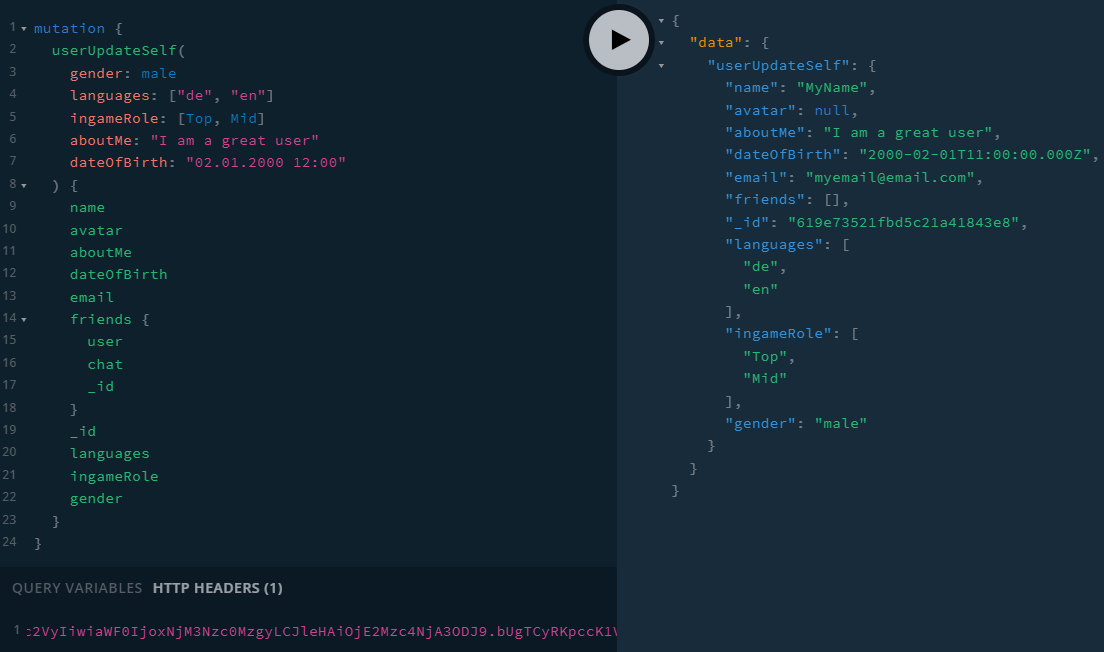
\includegraphics[width=\textwidth]{sources/graphiql_userUpdateSelf.png}
	\caption{Das Geschlecht, Sprachen, Rolle etc. für den aktiven Nuter werden gesetzt. Unten: Ausschnitt des Autorisierungstokens. Durch das Token wird der aktive Nutzer identifiziert. Eigene Darstellung.}
	\label{fig:gql:4}
\end{figure}

Zum Finden von neuen Nutzern wird die Abfrage \textit{userManyToSwipe} verwendet. Dabei werden dem abfragendem Nutzer durch einen Algorithmus die Profile von mehreren Nutzern geladen, die sich nicht bereits in der Freundesliste befinden oder vom aktiven Nutzer blockiert wurden.
Nutzer, welche dem aktiven Nutzer eine Freundesanfrage geschickt haben, werden präferiert gezeigt, um die Chance neuer Freundschaften zu erhöhen.
Es ist möglich, durch Filter die Menge der potenziellen Nuter zu reduzieren.
Im Frontend werden die Profile nacheinander angezeigt.
Es wäre möglich gewesen,  mit jeder Abfrage nur einen einzelnen Nutzer anzuzeigen.
Da das Laden von mehreren Nutzern pro Abfrage jedoch die Zahl der Abfragen stark erhöht, wurde sich dagegen entschieden.
Mit der Mutation \textit{swipe} kann dann eine Freundschaftsanfrage an den angegebenen Nutzer geschickt werden.

\begin{figure}
	\centering
    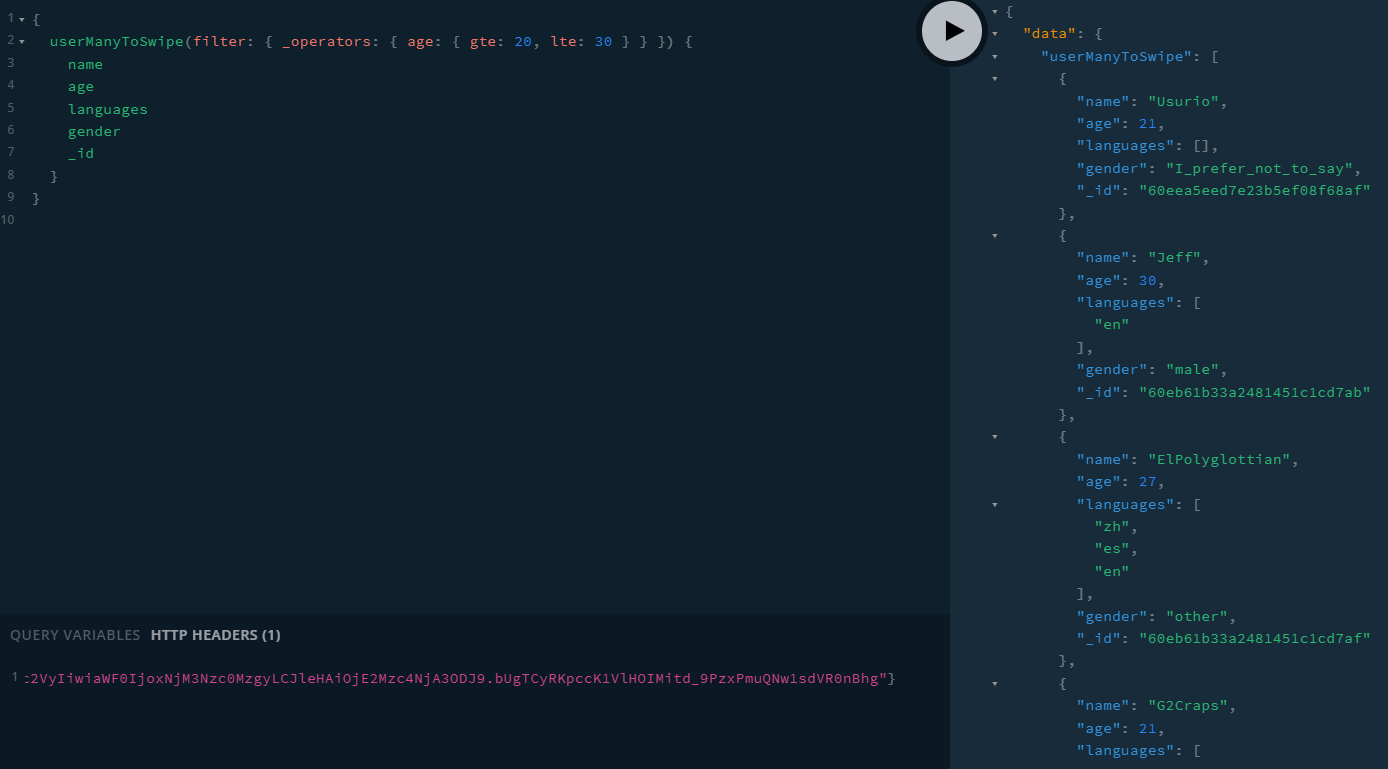
\includegraphics[width=\textwidth]{sources/graphiql_userManyToSwipe.png}
	\caption{Abfrage nach mehreren Nutzern mit userManyToSwipe. Durch den Filter werden nur Nutzer im Alter zwischen 20 und 30 Jahren angezeigt. Eigene Darstellung.}
	\label{fig:gql:5}
\end{figure}

\begin{figure}
	\centering
    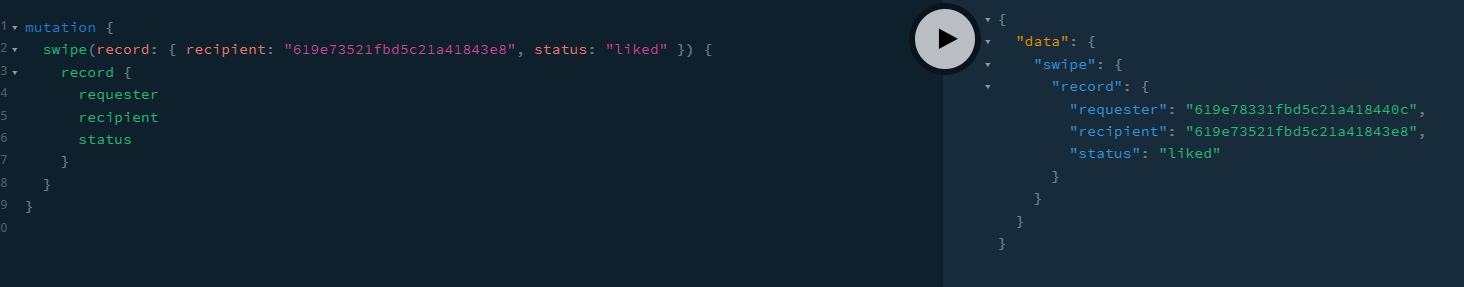
\includegraphics[width=\textwidth]{sources/graphiql_swipe.png}
	\caption{Der aktive Nutzer versendet einen Like an den durch \textit{recipient} definierten Nutzer. Eigene Darstellung.}
	\label{fig:gql:6}
\end{figure}

Die Nachrichten eines Chats können durch die Abfrage \textit{getChat} gelesen werden.
Dazu ist die ID des Chat anzugeben.
Der optionale Parameter „Seite“ gibt an, welche Nachrichten zurückgegeben werden sollen.
Auf jeder Seite befinden sich 20 Nachrichten, beginnend bei \enquote{Seite=1} mit den neuesten 20 Nachrichten.
Sollte der Seitenparameter nicht angegeben werden, wird nur die neueste Nachricht geladen.
Dies wird bei der Vorschau des Chats für die Freundesliste verwendet.

\begin{figure}
	\centering
    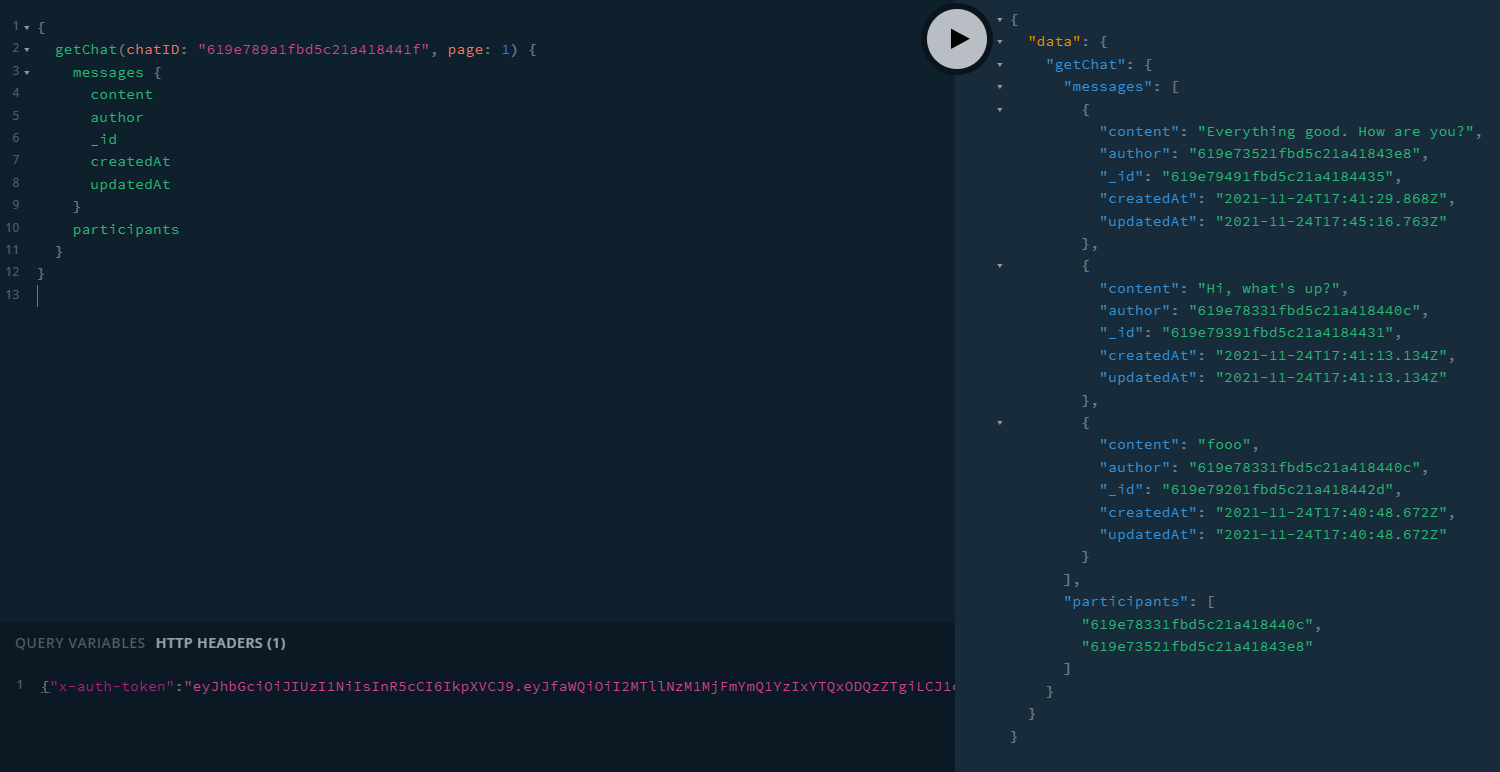
\includegraphics[width=\textwidth]{sources/graphiql_getChat.png}
	\caption{Durch den Parameter \textit{page: 1} werden die bis zu 20 letzten Nachrichten geladen. Da der Chat nur 4 Nachrichten beinhaltet werden nur diese geladen. Unten: Das Authentifizierungstoken \textit{x-auth-token} befindet sich in dem HTTP-Header der Abfrage. Eigene Darstellung.}
	\label{fig:gql:7}
\end{figure}

Mit \textit{sendMessage} können Nachrichten versendet werden. Dazu ist die ID des Chats notwendig.
Der im Parameter \textit{Inhalt} definierte Text wird dann in den Chat als neueste Nachricht versendet.
Um eine Nachricht zu editieren  oder zu löschen, ist die Mutation \textit{editOrDeleteMessage} zu verwenden.
Zusätzlich zur Chat-ID ist die Nachrichten-ID der zu verändernden Nachricht anzugeben. Der optionale Parameter \textit{content} gibt im Falle einer Änderung den neuen Nachrichteninhalt an.
Sollte \textit{content} nicht definiert sein, wird die gewählte Nachricht stattdessen gelöscht. 

\begin{figure}
	\centering
    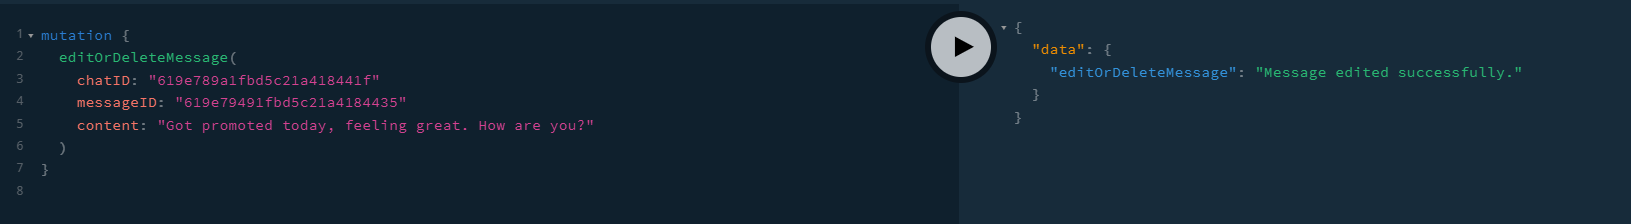
\includegraphics[width=\textwidth]{sources/graphiql_editMessage.png}\cite{}
	\caption{Die bestehende Nachricht (Siehe Abfrage \textit{getChat}) wird durch den in \textit{content} definierten Text ersetzt. Eigene Darstellung.}
	\label{fig:gql:8}
\end{figure}

\begin{figure}
	\centering
    \includegraphics[width=\textwidth]{sources/graphiql_deleteMessage.png}\cite{}
	\caption{Die soeben editierte Nachricht wird gelöscht. Eigene Darstellung.}
	\label{fig:gql:9}
\end{figure}

\subsection*{Fazit}
Es konnte gezeigt werden, dass GraphQL eine geeignete Wahl für das Projekt ist.
Neben den Anforderungen, welche auch durch eine REST-Schnittstelle gelöst werden könnten, glänzt GraphQL mit den genannten Vorteilen wie Leistungsoptimierungen, Stabilität und Selbstdokumentation.
Die gewählten Resolver ermöglichen einen einfachen Zugriff auf die auf der Datenbank liegenden Informationen und GraphiQL ermöglicht einen genauen Umgang mit der Schnittstelle.
Das Hochladen von Bilddateien stellt GraphQL vor eine Herausforderung, dieses Problem lässt sich jedoch mit dem zurückgreifen auf klassische REST-API lösen.